Here, a comparison of adaptive strategies is performed for the $Re=40,000$ case.
%, at advance ratio of $\mu_{sect}=1.2$, at an angle of attack of $\alpha=6^\circ$.
The three VMS-based error estimator driven mesh adaptation strategies considered here are zonal-based refinement, nodal size field-based adaptation, and feature-based refinement. Phase-averaged flow data is used, and the maximum local error taken over multiple phases and over the spanwise direction is used as a representation for the entire surging cycle. In particular, we consider 24 phases that are regularly spaced over the cycle and includes the end of the cycle. 

\subsection{Zonal Refinement}
In this strategy, an initial solution is obtained on an initial mesh with a set of canonical refinement zones that are usually used for a flow over an airfoil. We refer to this mesh as M0\_nz25, see Figure \ref{fig:M0_mesh}. In-plane mesh sizes are indicated in the figure. The initial mesh spacing/resolution on the surface of the airfoil in the streamwise and spanwise directions is set to be below 75 and 40 in wall units, respectively.
Here nz25 refers to the number of spanwise extruded layers (i.e., 25) used in this mesh. 
As mentioned before, the VMS-based error estimator is applied to phase-averaged data, and the maximum error value over multiple phases (i.e., at 24 equispaced phases over the surging cycle), and over the spanwise direction, is selected to represent the element-level local error within the airfoil plane/section throughout the surging cycle. 
The element-level error estimated on this mesh is shown in Figure \ref{fig:M0_err_plot}. 
We can see that higher errors are observed primarily in the regions traversed by the LEV through the surging cycle, as well as in the wake of the airfoil. 
Higher errors are also observed close to the airfoil surface and in the boundary layer region.

Based on the estimated error, the mesh is refined by a factor of 2 in zones where high error values are found, including in the boundary layer mesh (i.e., along the streamwise direction). 
The spanwise resolution is also refined by a factor of 2 (i.e., the number of layers in the spanwise direction is doubled). 
This adapted mesh is shown in Figure \ref{fig:Mza1_mesh} and the estimated error on it is shown in Figure \ref{fig:Mza1_err_plot}. It is referred to as the Mza1\_nz50 mesh (where za is short for zonal adaptation and 1 in za1 denotes the first iteration of mesh adaptation).
%It is observed that the error has approximately reduced by a factor of 4 in the Mza1\_nz50 mesh as compared to the M0 mesh.
It is observed that the error has reduced in the Mza1\_nz50 mesh as compared to the M0 mesh
These meshes, M0\_nz25 and Mza1\_nz50, consist of 774,525 and 2,874,300 elements, respectively.

%Zonal refinements are added to the Mza1 mesh in regions of high error, and the mesh is refined further by a factor of 2 in these zones, along with the boundary layer mesh in the streamwise direction, and the number of layers in the spanwise direction is doubled.  This mesh, which is referred to as Mza2, is shown in Figure \ref{fig:Mza2_mesh}. Again, we observe that the error has reduced by a factor of 4 in the Mz\_a2 mesh as compared to Mz\_a1 mesh.

%The number of elements for each mesh is presented in Table \ref{table:mesh_zonal_summary}.


% \begin{table}[H]
% 	\centering
% 	\caption{Summary of zonal refinement based meshes}
% 	\label{table:mesh_zonal_summary}
% 	\begin{tabular}{|l|c|c|c|c|c|}
% 		\hline
% 		Mesh case  & No. of elements\\
% 		\hline
% 		\hline
% 		M0\_nz25 & 774,525 \\
% 		\hline
% 		Mza1\_nz50 &  2,874,300 \\
% 		\hline
% %		Mz\_a2 & 14,329,200 \\
% %		\hline
% 	\end{tabular}
	
% \end{table}

A comparison of different adaptive strategies/adapted meshes is provided in Section \ref{sec:results_adapt}.

\begin{figure}[H]
\centering
\begin{subfigure}[b]{0.475\textwidth}
\centering
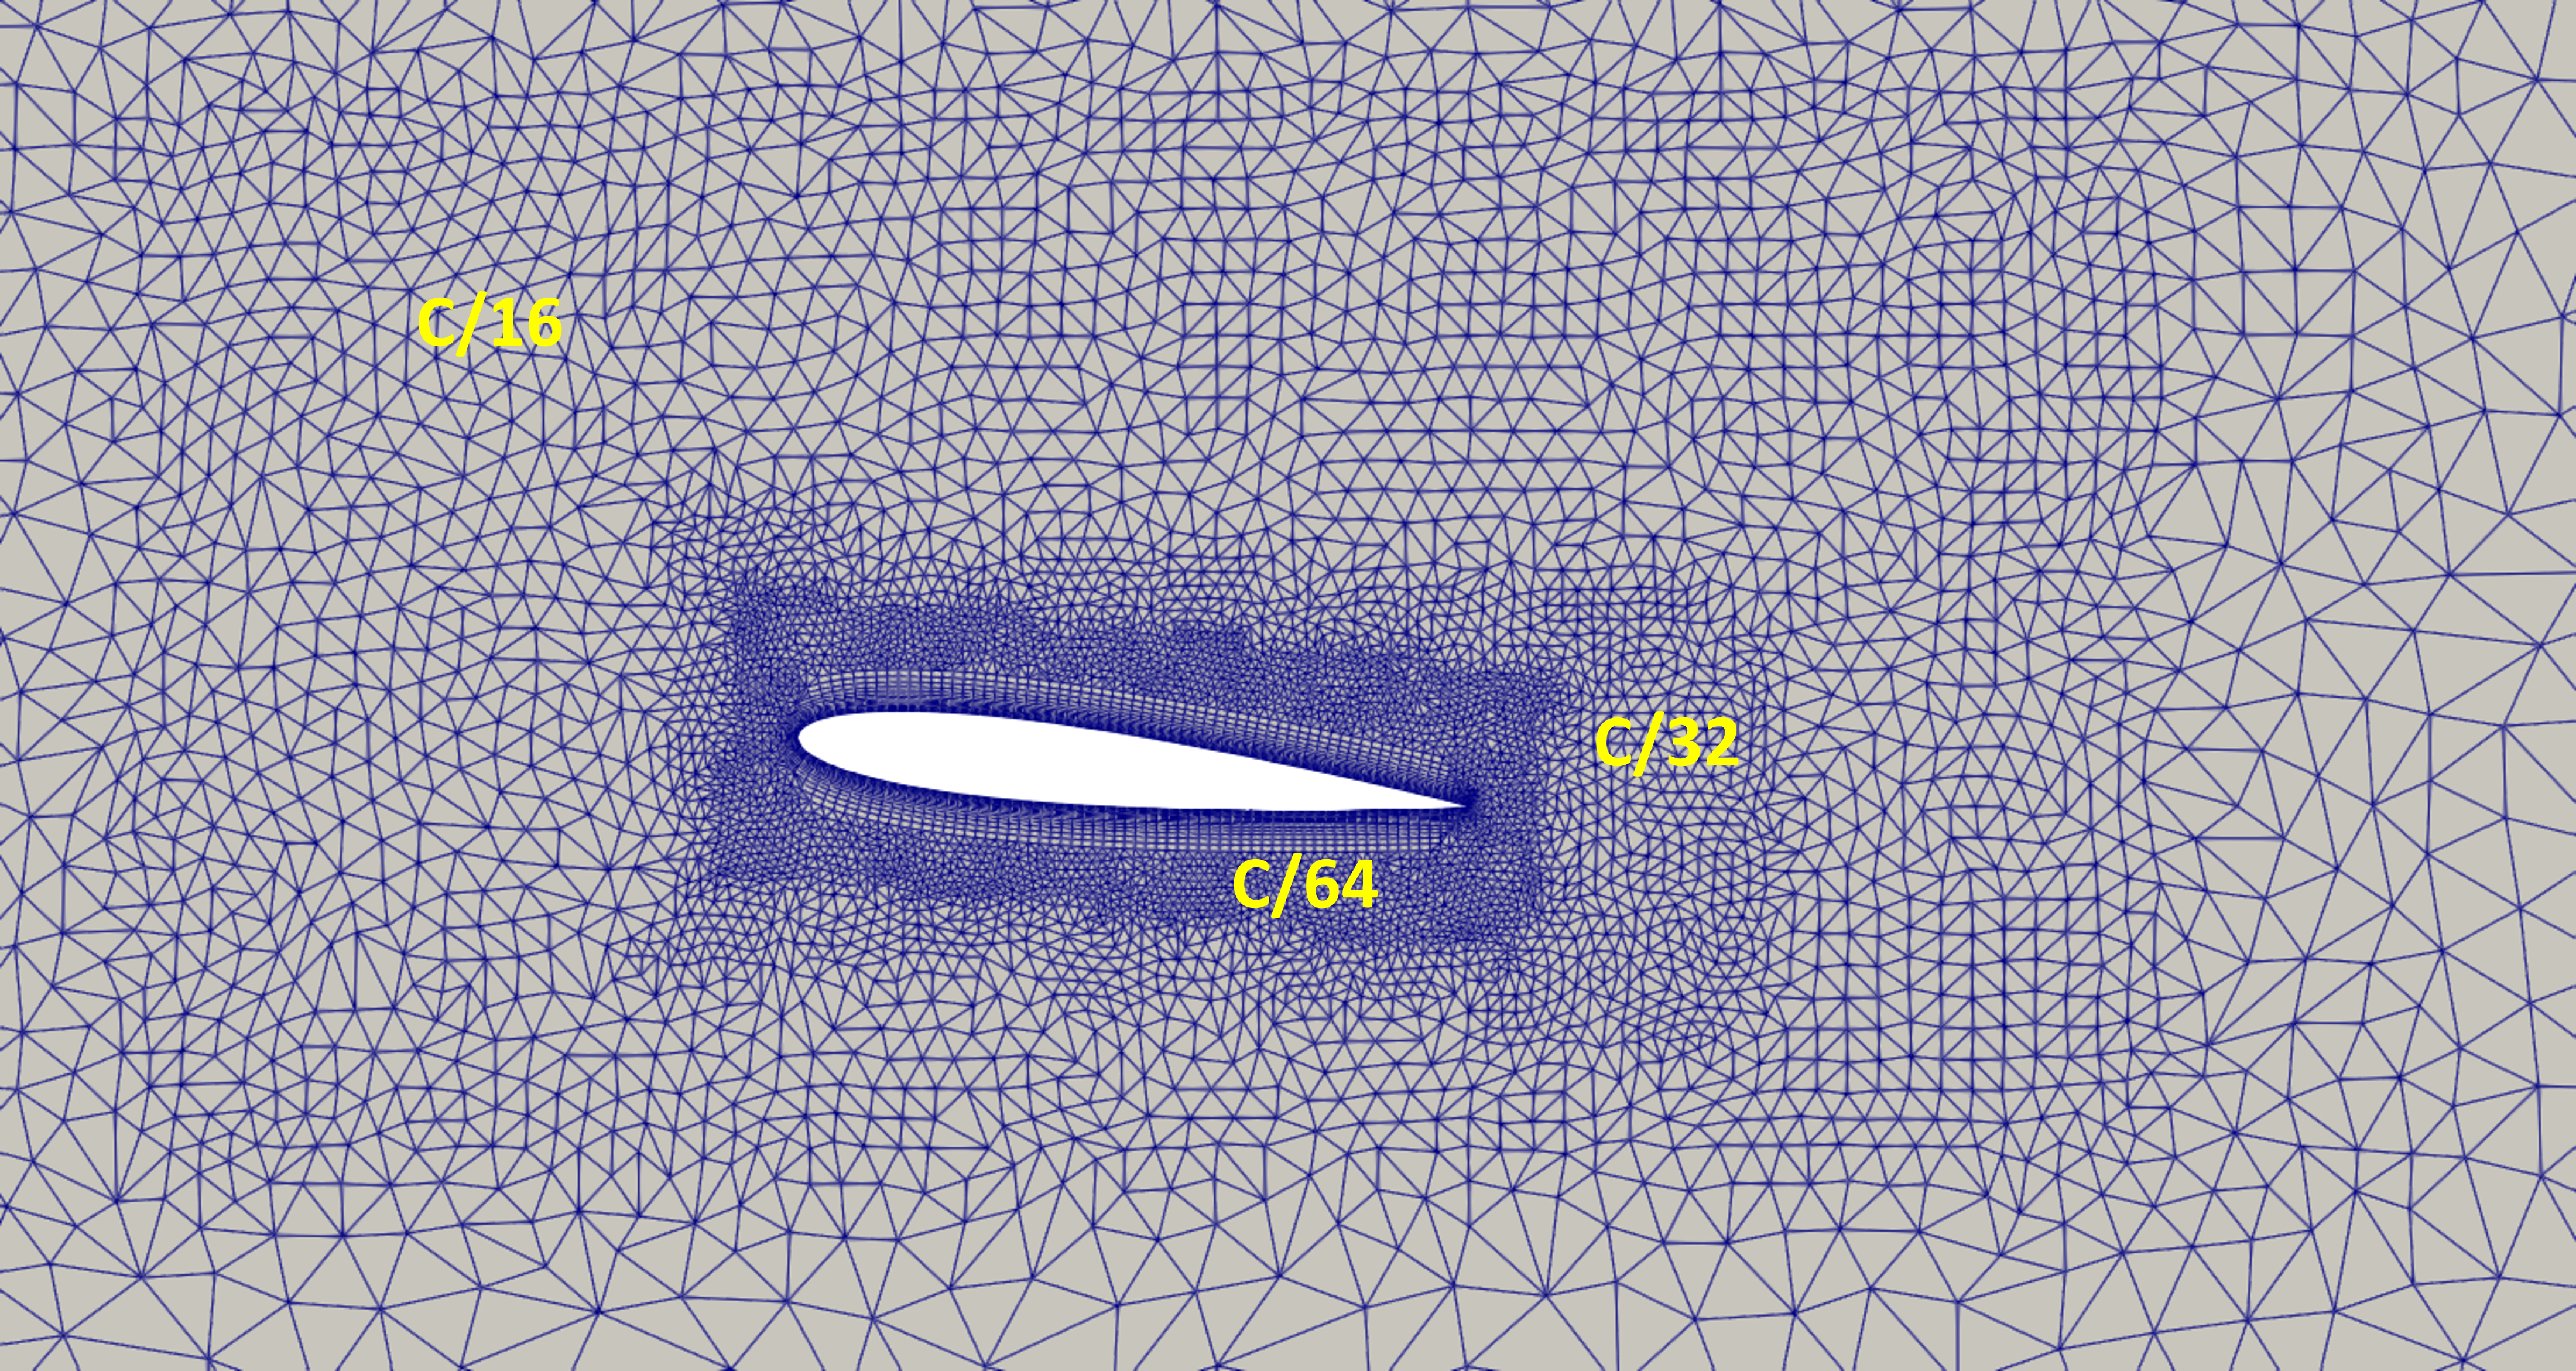
\includegraphics[width=1\textwidth]{figures/adapt_strat/M0_mesh.png}
\caption{M0\_nz25 mesh}
\label{fig:M0_mesh}
\end{subfigure}
\begin{subfigure}[b]{0.475\textwidth}
\centering
\includegraphics[width=1\textwidth]{figures/adapt_strat/M0_error.png}
\caption{M0\_nz25 error field}
\label{fig:M0_err_plot}
\end{subfigure}
\begin{subfigure}[b]{0.475\textwidth}
\centering
\includegraphics[width=1\textwidth]{figures/adapt_strat/Mza1_mesh.png}
\caption{Mza1\_nz50 mesh}
\label{fig:Mza1_mesh}
\end{subfigure}
\begin{subfigure}[b]{0.475\textwidth}
\centering
\includegraphics[width=1\textwidth]{figures/adapt_strat/Mza1_error.png}
\caption{Mza1\_nz50 error field}
\label{fig:Mza1_err_plot}
\end{subfigure}
%\begin{subfigure}[b]{0.475\textwidth}
%\centering
%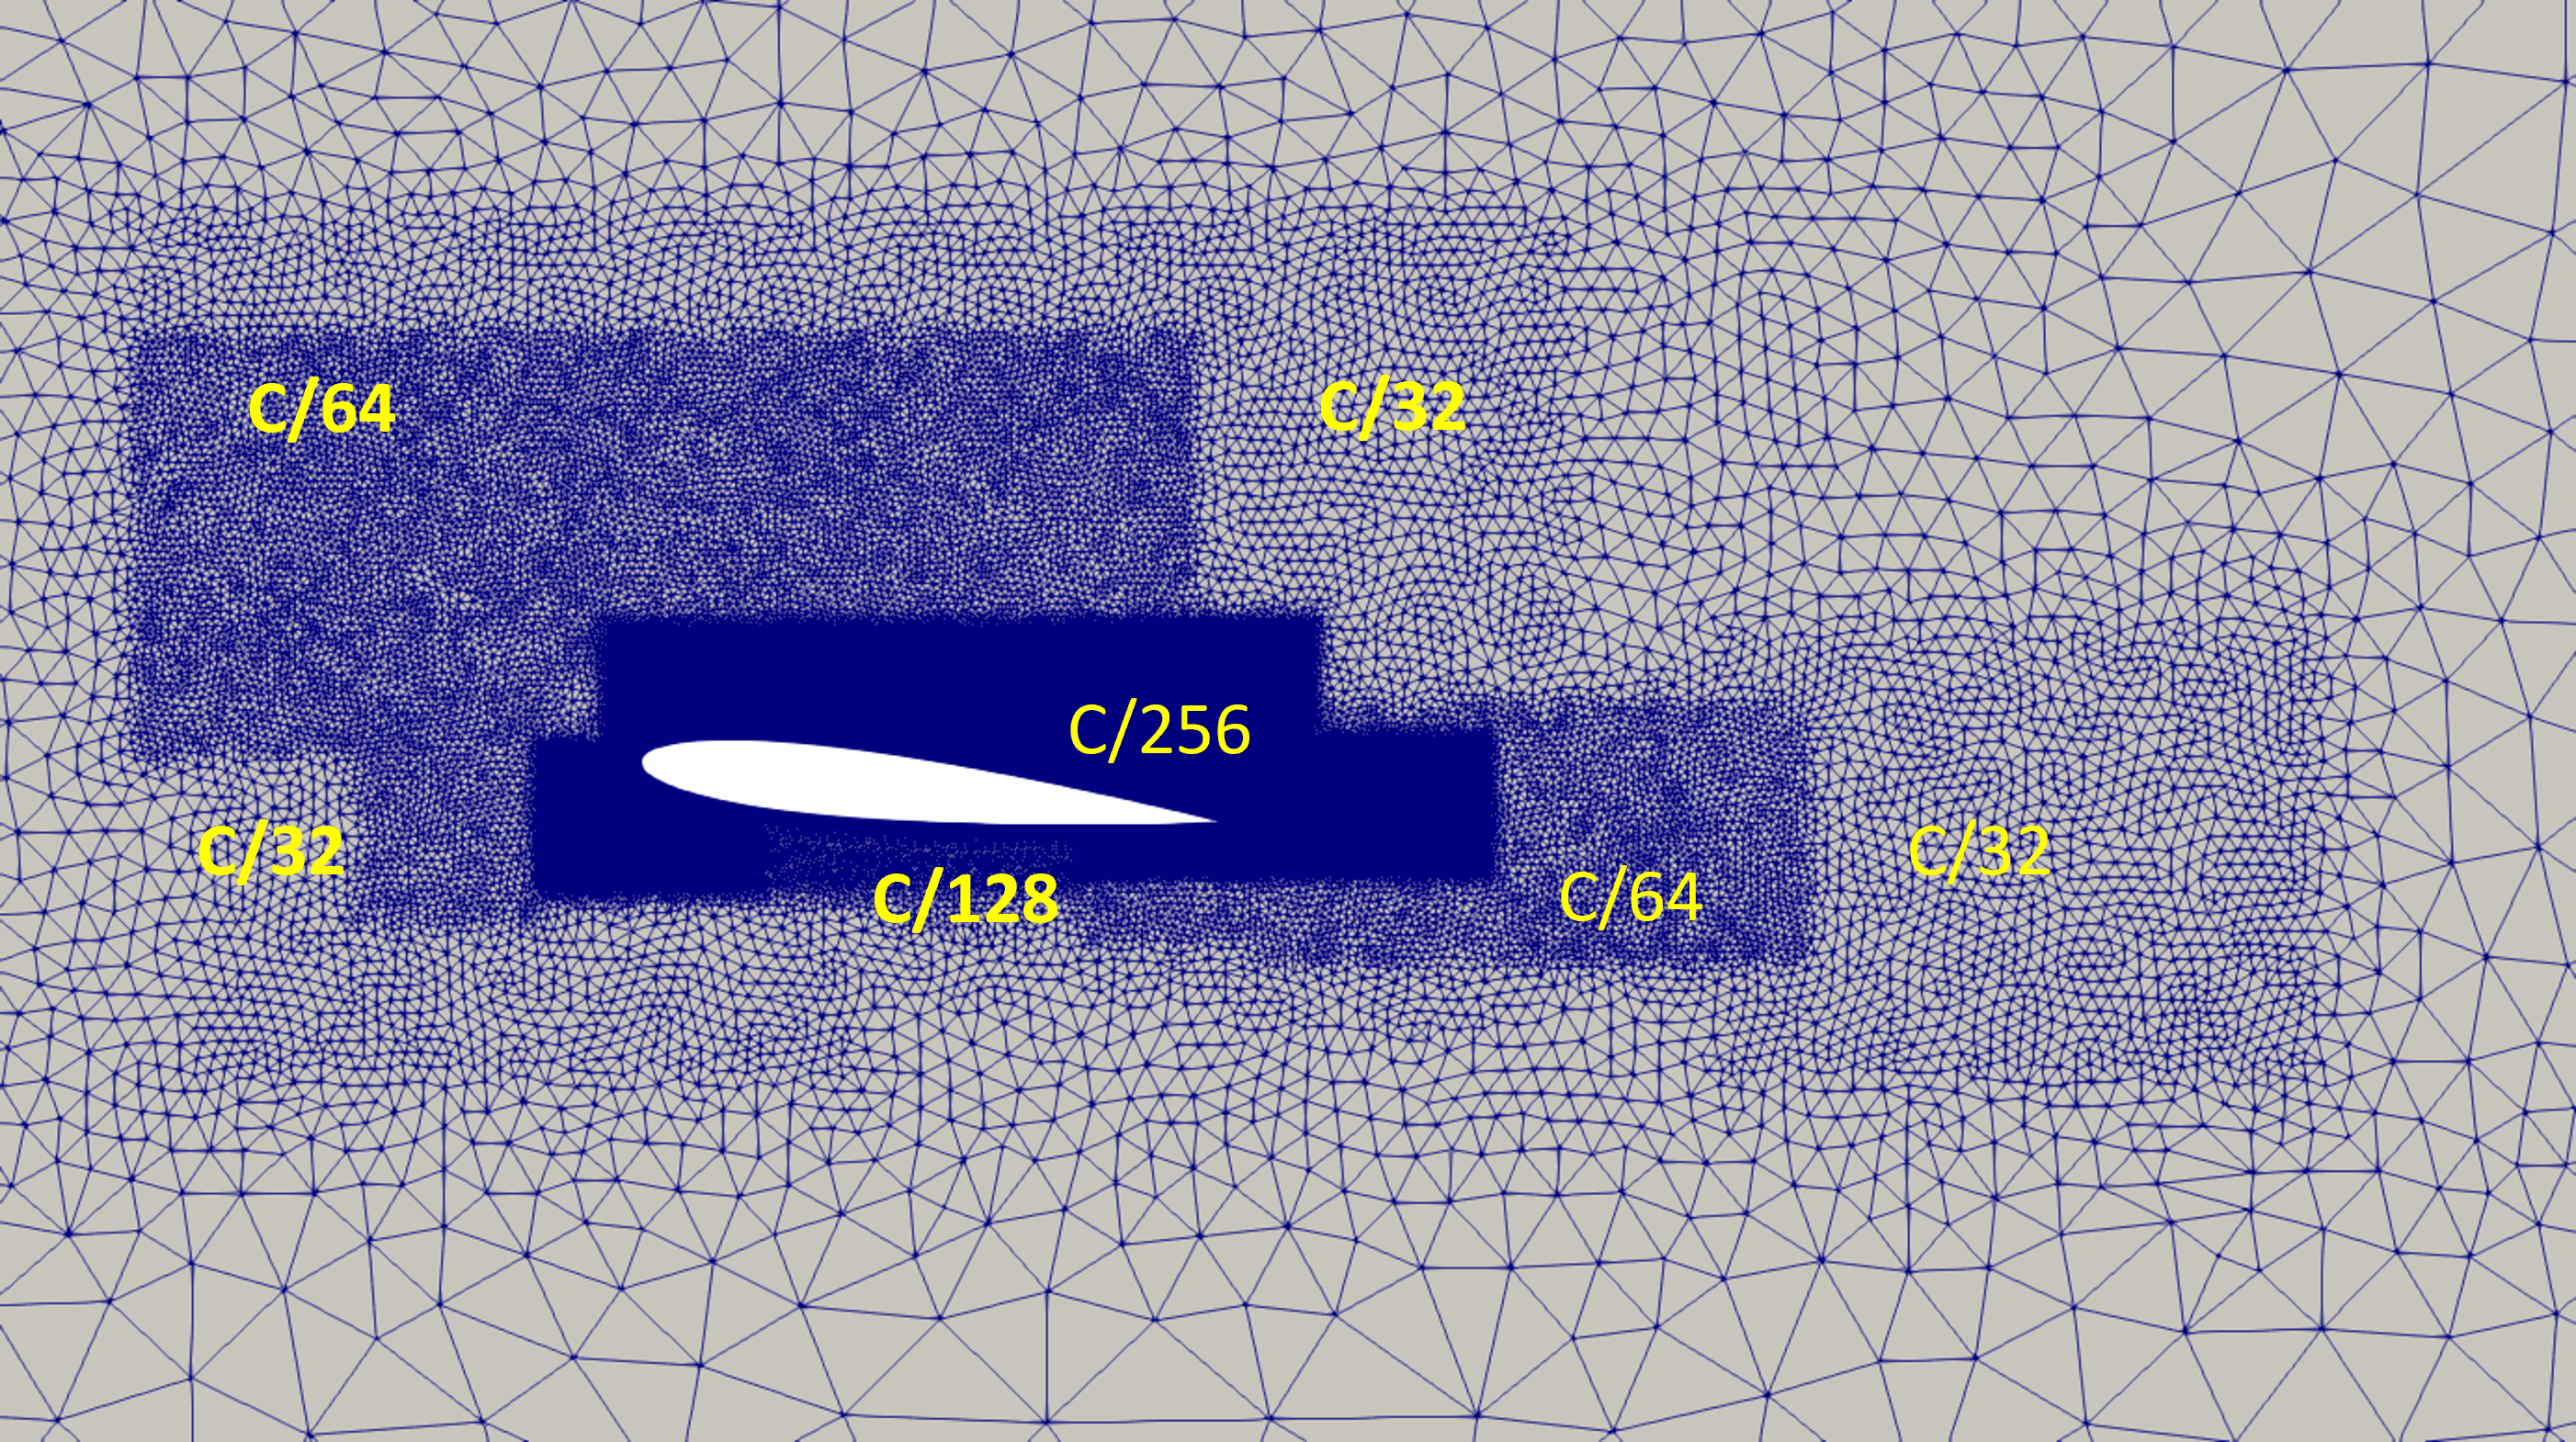
\includegraphics[width=1\textwidth]{figures/adapt_strat/Mza2_mesh.png}
%\caption{Mz\_a2 mesh}
%\label{fig:Mza2_mesh}
%\end{subfigure}
%\begin{subfigure}[b]{0.475\textwidth}
%\centering
%\includegraphics[width=1\textwidth]{figures/adapt_strat/Mza2_error_plot.png}
%\caption{Mz\_a2 error field}
%\label{fig:Mza2_err_plot}
%\end{subfigure}
\caption{Meshes and estimated error fields for zonal-based strategy}
\end{figure}



\subsection{Nodal Size Field-based Adaptation}
In this adaptive strategy, the VMS-based error is calculated on the initial mesh. Based on the estimated error, a nodal size field is calculated using the Equation \eqref{eq:diez}, see Section \ref{sec:sf_adapt}.

% \begin{equation}
% \frac{e_k}{\tilde{e}_k} = \left(\frac{h_{old}}{h_{new}}\right)^{m+N/2} 
% \label{eq:diez}
% \end{equation}

%Here, $e_k$ is the measured local error (in the $\HOne$-seminorm) at an element $k$, $\tilde{e}_k$ is the target error for an element specified by the user, $m$ is the polynomial order of the approximation space (i.e., $m=1$ for the linear finite elements used currently) , and $N$ is the number of spatial dimensions. $h_{old}$ is current size of the element, and $h_{new}$ is the desired new mesh size.
%This new mesh size at the element level is assembled at the node/vertex level to perform mesh adaptation.

\begin{figure}[H]
\centering
\begin{subfigure}[b]{0.475\textwidth}
\centering
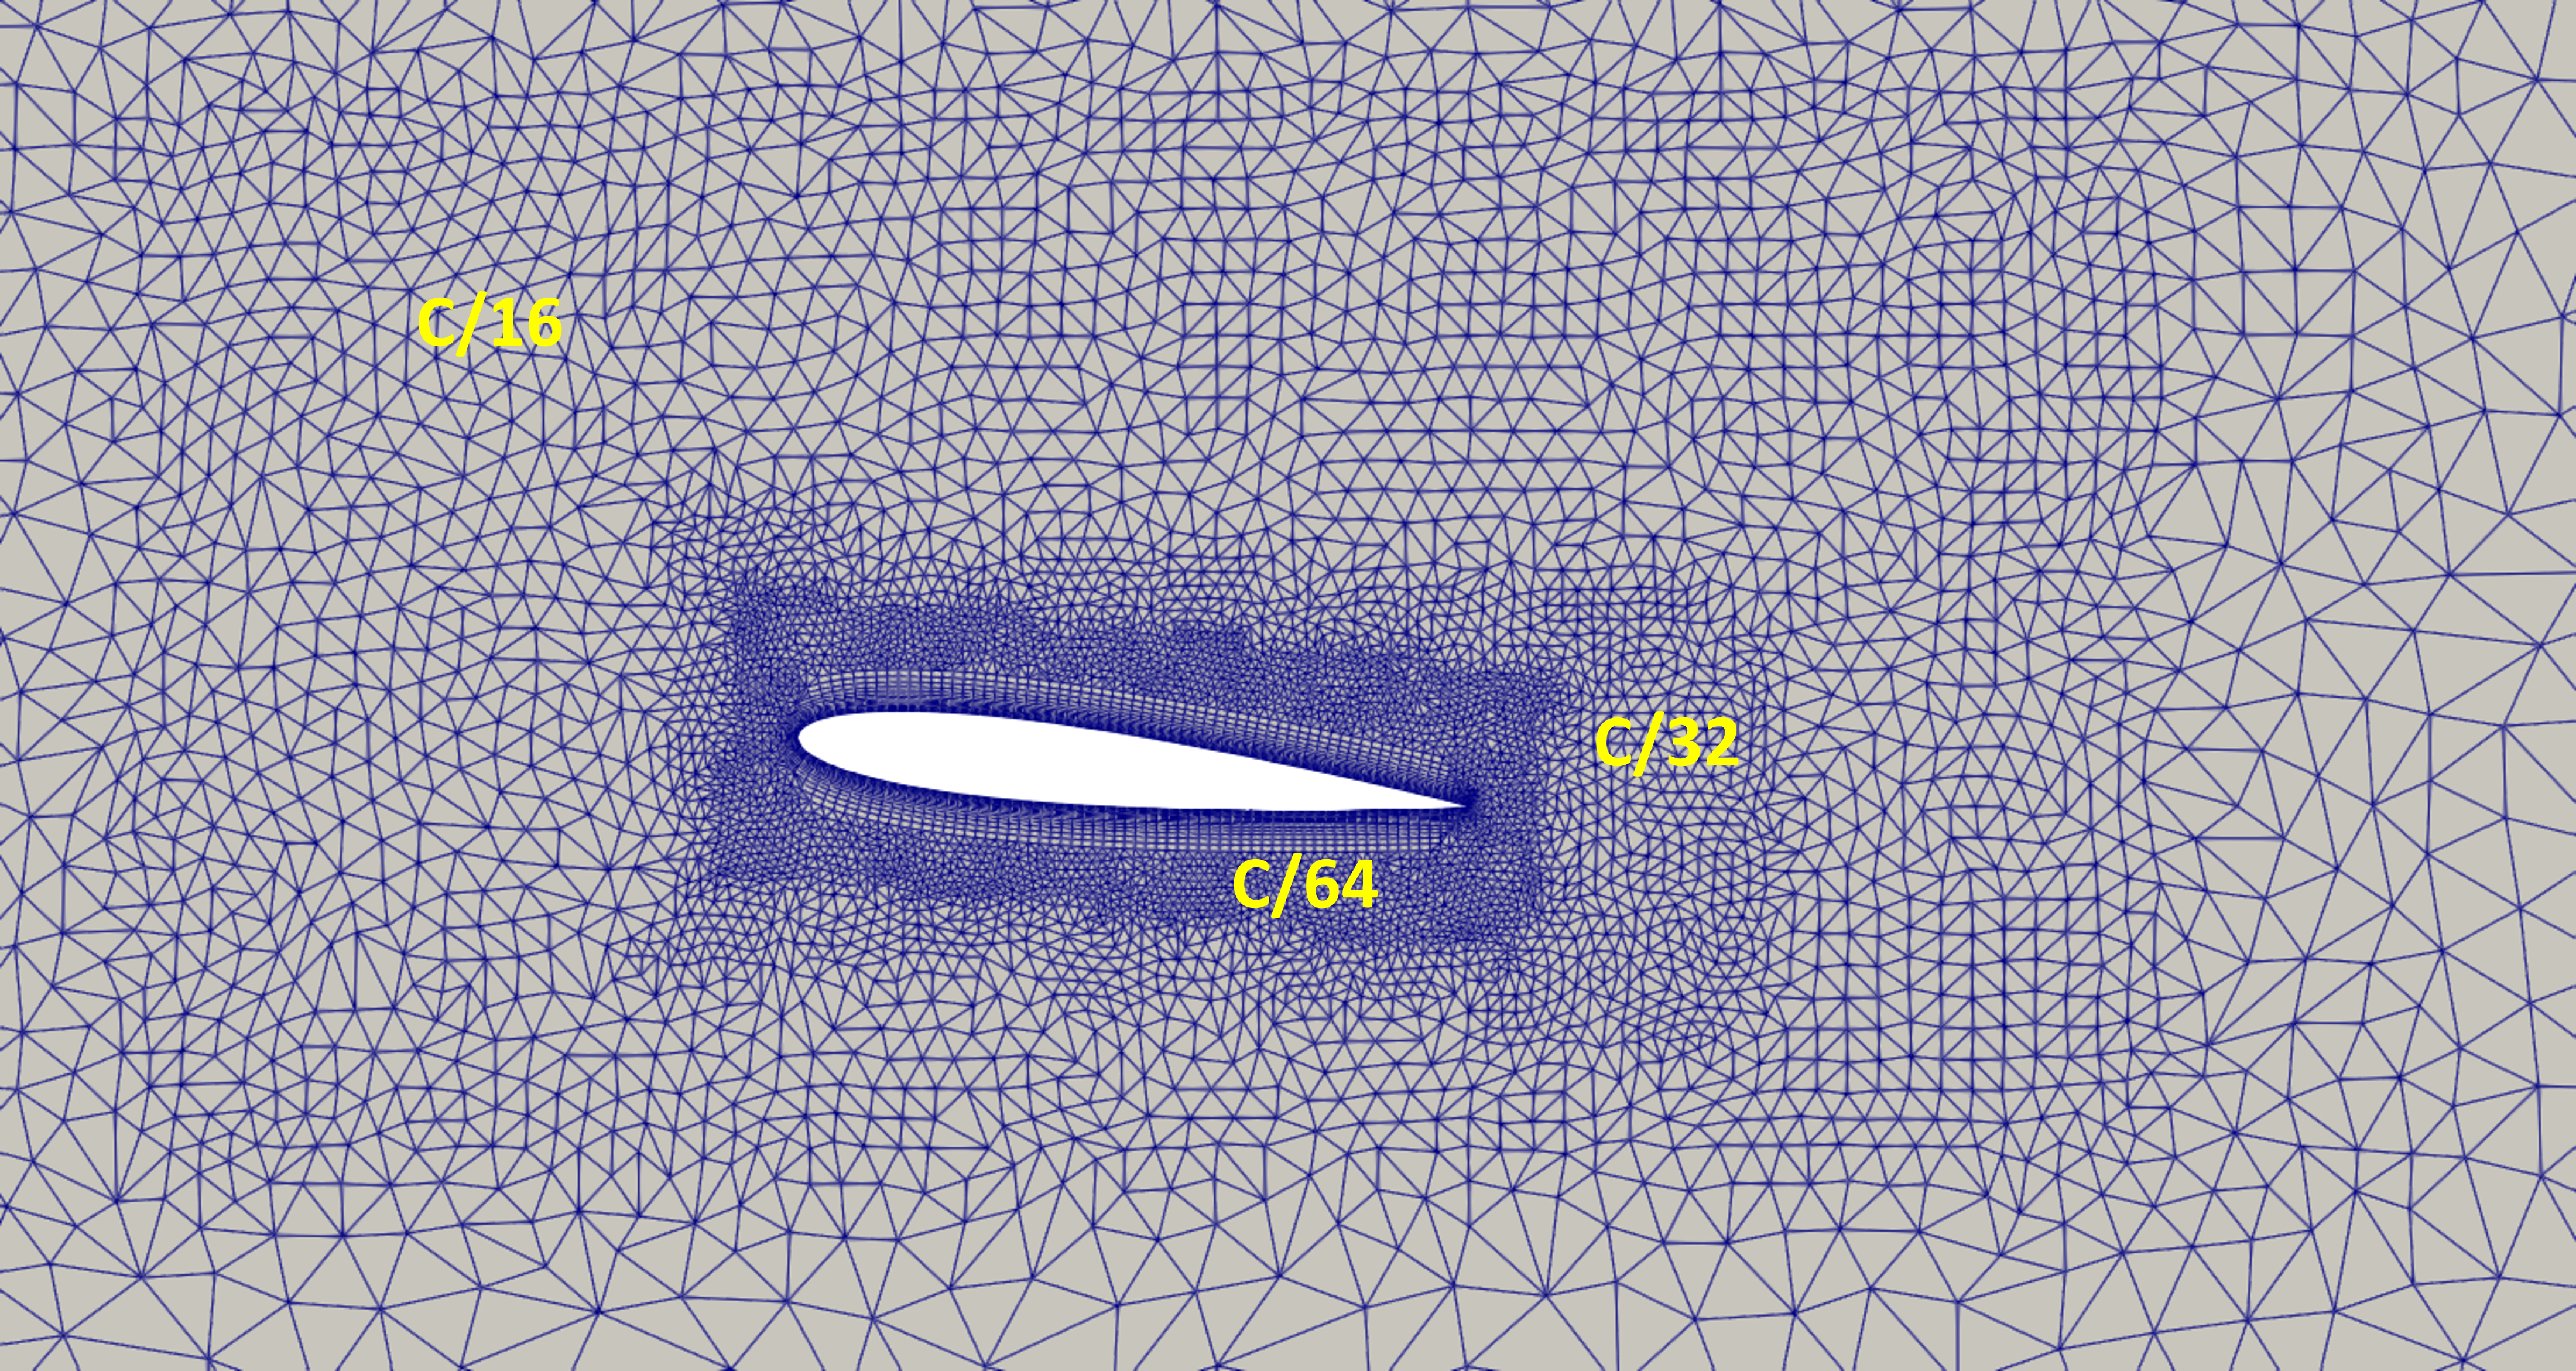
\includegraphics[width=1\textwidth]{figures/adapt_strat/M0_mesh.png}
\caption{M0\_nz25 mesh}
\label{fig:M0_mesh_sa}
\end{subfigure}
\begin{subfigure}[b]{0.475\textwidth}
\centering
\includegraphics[width=1\textwidth]{figures/adapt_strat/M0_error.png}
\caption{M0\_nz25 error field}
\label{fig:M0_err_plot_sa}
\end{subfigure}
\begin{subfigure}[b]{0.475\textwidth}
\centering
\includegraphics[width=1\textwidth]{figures/adapt_strat/Msa1_mesh.png}
\caption{Msa1\_nz50 mesh}
\label{fig:h_adapt1_mesh}
\end{subfigure}
\begin{subfigure}[b]{0.475\textwidth}
\centering
\includegraphics[width=1\textwidth]{figures/adapt_strat/Msa1_error.png}
\caption{Msa1\_nz50 error field}
\label{fig:h_adapt1_error_plot}
\end{subfigure}

\caption{Meshes and estimated error fields for size-based strategy}
\end{figure}

As before, M0\_nz25 is used as the initial mesh (Figure \ref{fig:M0_mesh}) and the corresponding error estimated on M0\_nz25 mesh (Figure \ref{fig:M0_err_plot}) is used to calculate nodal size field (i.e., $h_{new}$ at every mesh node/vertex). The mesh adaptation is limited or controlled to have a maximum refinement and maximum coarsening by a factor of 2 to avoid excessive refinement or coarsening in any local region. The number of extruded layers in the spanwise direction are doubled to 50. The adapted mesh obtained using this strategy is shown in Figure \ref{fig:h_adapt1_mesh}. It is referred to as the Msa1\_nz50 mesh (where sa is short for size-based adaptation and 1 in sa1 denotes the first iteration of mesh adaptation). Note that in terms of mesh resolution, this adapted mesh, Msa1\_nz50, compares well against the Mza1\_nz50 mesh obtained from the zonal-based strategy. Msa1\_nz25 mesh consists of 2,859,450 elements, which is comparable to 2,874,300 elements for the Mza1\_n50 mesh. The major differences between the two meshes is that Mza1\_nz50 maintains the same mesh size in various zones, whereas mesh size varies locally (even within a zone) in Msa1\_nz50.
The corresponding estimated error for this mesh is shown in Figure \ref{fig:h_adapt1_error_plot}. M0\_nz0 mesh and error field are shown again to compare against Msa1\_nz50. Comparing the estimated error between the Msa1\_nz50 and Mza1\_nz50 meshes, higher error values are observed in the LEV regions as well as in the wake of the airfoil. Overall, the estimated error on the Msa1\_nz50 mesh is higher as compared to that on the Mza1\_nz50 mesh. A more detailed comparison of different adaptive strategies/adapted meshes is provided in Section \ref{sec:results_adapt}.


\subsection{Feature-based Refinement}
In this strategy, mesh refinement is applied around the dominant flow features of interest.
In the current surging airfoil case, LEV is the dominant flow feature. 
Using vortex detection and tracking (see Section \ref{sec:LEV_detect_track}), LEV evolution (path and size) is determined using an initial mesh (M0\_nz25 in this case). 
Based on this a refinement zone is added around the path of the LEV.
In such a feature-based refinement, VMS-based estimated error is used to set the mesh size in the refinement zone(s) around the dominant feature(s). 
In addition, estimated error is also used to refine the mesh around the airfoil (e.g., in a similar fashion as the error-based zonal refinement discussed earlier). 
This is done to accurately resolve the flow near the airfoil including the boundary layer region that plays a direct role in the formation of LEV.

In summary, the mesh around the LEV path is refined by a factor of 2. In addition, the boundary layer mesh is refined by a factor of 2 in the streamwise direction, and again, the number of layers in the spanwise direction are doubled as compared to M0\_nz25.
The resulting mesh resolution on the surface of the airfoil in the streamwise and spanwise directions is below 40 and 25 in wall units, respectively, i.e., same as the previous cases.
This adapted mesh is referred to as the Mfa1\_nz50 mesh (where fa is short for feature-based adaptation and 1 in fa1 denotes the first iteration of mesh adaptation). 
This mesh is shown in Figure \ref{fig:FB_mesh} and the estimated error on it is shown in Figure \ref{fig:FB_error_plot}.
M0\_nz0 mesh and error field are shown again to compare against Mfa1\_nz50.
Mfa1\_nz50 contains 2,777,750 elements, which is comparable to both Mza1\_nz50 and Msa1\_nz50 meshes.

Error values are similar to those obtained on the Mza1\_nz50 mesh, i.e., near the airfoil surface, in the LEV path, and in the wake, since mesh resolution in crucial regions is similar between the Mfa1\_nz50 and Mza1\_nz50 meshes, while estimated error is higher on the Msa1\_nz50 mesh.
%Error values are lower as compared to Msa1\_nz50, since a uniform mesh size is maintained, as opposed to Msa1\_nz50, where the mesh size is patchy.
A more detailed comparison of different adaptive strategies/adapted meshes is provided in Section \ref{sec:results_adapt}.

\begin{figure}[H]
\centering
\begin{subfigure}[b]{0.475\textwidth}
\centering
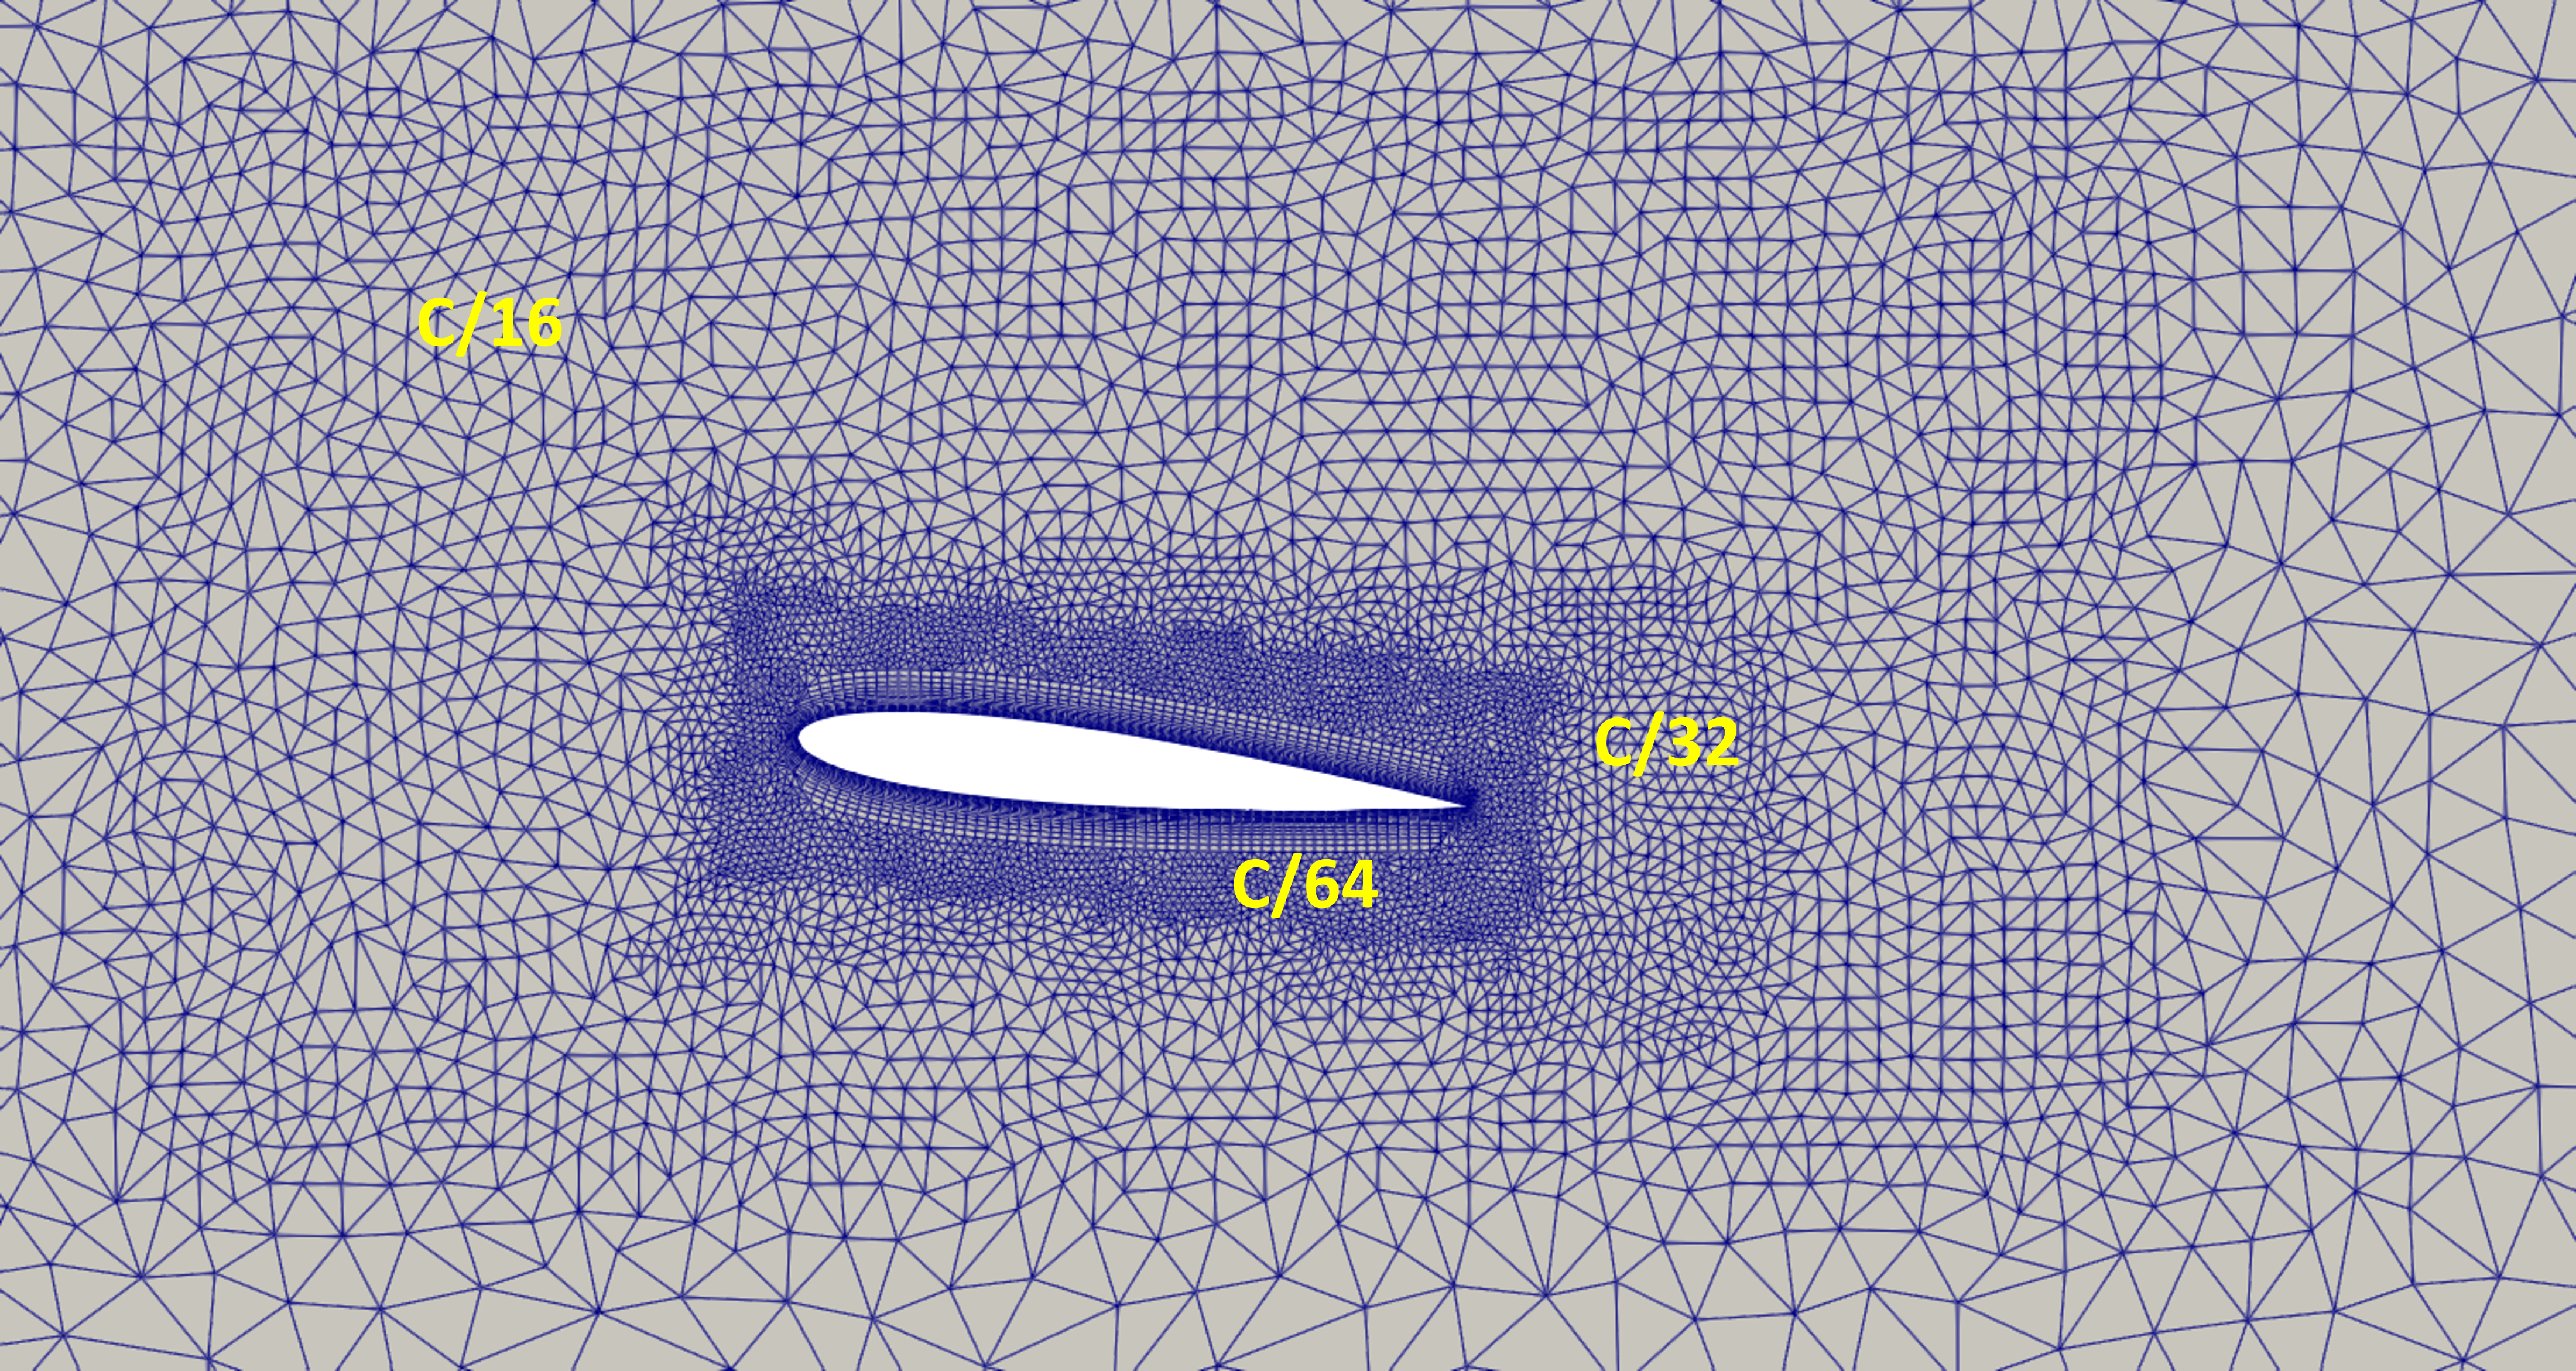
\includegraphics[width=1\textwidth]{figures/adapt_strat/M0_mesh.png}
\caption{M0\_nz25 mesh}
\label{fig:M0_mesh_fa}
\end{subfigure}
\begin{subfigure}[b]{0.475\textwidth}
\centering
\includegraphics[width=1\textwidth]{figures/adapt_strat/M0_error.png}
\caption{M0\_nz25 error field}
\label{fig:M0_err_plot_fa}
\end{subfigure}
\begin{subfigure}[b]{0.475\textwidth}
\centering
\includegraphics[width=1\textwidth]{figures/adapt_strat/Mfa1_mesh.png}
\caption{Mfa1\_nz50 mesh}
\label{fig:FB_mesh}
\end{subfigure}
\begin{subfigure}[b]{0.475\textwidth}
\centering
\includegraphics[width=1\textwidth]{figures/adapt_strat/Mfa1_error.png}
\caption{Mfa1\_nz50 error field}
\label{fig:FB_error_plot}
\end{subfigure}

\caption{Meshes and estimated error fields for feature-based strategy}
\end{figure}
\label{sec:feature_based_strat}


\subsection{Comparison}
In this section, we compare results of different adapted meshes obtained from three adaptive strategies mentioned above. 
We compare different quantities of interest. 
A comparison of force response in the form of normalized lift and drag forces is shown in Figures \ref{fig:lift_plot} and \ref{fig:drag_plot}, respectively. The normalized lift and drag matches up well for all the adapted meshes.

A comparison of spanwise vorticity for the different adapted meshes is shown in Figures \ref{fig:vorticity_195}, \ref{fig:vorticity_210} and \ref{fig:vorticity_270}, for 3 phases of $\psi=210^\circ$, $\psi=225^\circ$ and $\psi=270^\circ$, respectively.
For $\psi=195^\circ$, as the airfoil is in the retreating phase, boundary layer roll-up towards the geometric leading edge is observed over the airfoil surface.
For the meshes based on zonal refinement, as we go from M0\_nz25 to Mza1\_nz50, the separation over the airfoil is well resolved, and finer scales or flow structures are visible on the adapted mesh.
Comparing Mza1\_nz50, Msa1\_nz50, and Mfa1\_nz50 meshes, we can see that the Msa1\_nz50 mesh (sizefield-based adapted mesh) does not capture the finer scales/structures as compared to the Mza1\_nz50 mesh, both over the airfoil surface and in the wake of the airfoil, i.e., flow structures are more diffused in the case of Msa1\_nz50.
On the other hand, the Mfa1\_nz50 mesh captures them well.

\begin{figure}[H]
\centering

\begin{subfigure}[b]{0.7\textwidth}
\centering
\includegraphics[width=1\textwidth]{figures/Results/Lift_adapt_strat.png}
\caption{Normalized lift}
\label{fig:lift_plot}
\end{subfigure}
\begin{subfigure}[b]{0.7\textwidth}
\centering
\includegraphics[width=1\textwidth]{figures/Results/Drag_adapt_strat.png}
\caption{Normalized drag}
\label{fig:drag_plot}
\end{subfigure}

\label{fig:force_response_adapt}
\caption{Normalized forces for different adaptive strategies/adapted meshes}
\end{figure}

%Next, we look at the location of the LEV core for different meshes in Figure \ref{fig:LEV_location}. Some differences in the LEV location for various phases are observed. LEV location for Ma1, FB, and hadapt meshes is similar in the beginning phases. Ma1 starts to deviate from FB and hadapt in the later phases. LEV location for FB and hadapt meshes start to match with Ma2 in the later phases, whereas M0 LEV location fluctuates around the other meshes. This however is still not conclusive as to which mesh performs better and a more quantitative study is needed.


%%\begin{figure}[H]
%\centering
%\includegraphics[width=0.7\textwidth]{figures/Results/LEV_location.png}
%\caption{LEV location for different meshes}
%\label{fig:LEV_location}
%\end{figure}
%%


For $\psi=210^\circ$, formation of LEV begins to take place, as we start to see the roll-up of separated shear layer near the geometric leading edge. 
At this phase, the differences in the structures resolved by the different meshes become more clear.
Similar to $\psi=195^\circ$, the Msa1\_nz50 mesh shows a relatively poor resolution of the finer flow structures as compared to the Mza1\_nz50 and Mfa1\_nz50 meshes.

For $\psi=270^\circ$, differences can be seen in the separated shear layer at the geometric leading edge of the airfoil, and the resolution of the LEV, among different adapted meshes.
These are resolved better on the Mfa1\_nz50 and Mza1\_nz50 meshes. 
Recall that Mfa1\_nz50 is obtained using feature-based mesh refinement designed to capture the LEV accurately, and has the same mesh resolution as Mza1\_nz50 along the path of the LEV. 
%Once again, shear layer is not well resolved for Msa1\_nz50 as compared to other refined/adapted meshes.

The relatively poor resolution of flow, with more diffused flow structures, observed for Msa1\_nz50 can be attributed to the variation in mesh sizes (even by a factor of 1.5 or 2) in crucial regions of interest, i.e., the mesh size is not uniform or even quasi-uniform in particular zones. In particular, this seem to have an adverse effect in regions with turbulence.

\begin{figure}[H]
\centering
\begin{subfigure}[b]{0.475\textwidth}
\centering
\includegraphics[width=1\textwidth]{figures/adapt_strat/vorticity_plots/M0/phase_195.png}
\caption{M0\_nz25 mesh, $\psi$ = $195^\circ$}
\label{fig:M0_psi195}
\end{subfigure}
\begin{subfigure}[b]{0.475\textwidth}
\centering
\includegraphics[width=1\textwidth]{figures/adapt_strat/vorticity_plots/Mza1_50/phase_195.png}
\caption{Mza1\_nz50 mesh, $\psi$ = $195^\circ$}
\label{fig:Ma1_psi195}
\end{subfigure}
%\begin{subfigure}[b]{0.475\textwidth}
%\centering
%\includegraphics[width=1.25\textwidth]{figures/vorticity_plots/Mza2/ph_195.png}
%\caption{Mz\_a2 mesh, $\psi$ = $195^\circ$}
%\label{fig:Ma2_psi195}
%\end{subfigure}
\begin{subfigure}[b]{0.475\textwidth}
\centering
\includegraphics[width=1\textwidth]{figures/adapt_strat/vorticity_plots/Msa1_50/phase_195.png}
\caption{Msa1\_nz50 mesh, $\psi$ = $195^\circ$}
\label{fig:hadapt_psi195}
\end{subfigure}
\begin{subfigure}[b]{0.475\textwidth}
\centering
\includegraphics[width=1\textwidth]{figures/adapt_strat/vorticity_plots/Mfa1_50/phase_195.png}
\caption{Mfa1\_nz50 mesh, $\psi$ = $195^\circ$}
\label{fig:FB_psi195}
\end{subfigure}
\caption{Spanwise vorticity comparison at $\psi$ = $195^\circ$ for different adaptive strategies/adapted meshes}
\label{fig:vorticity_195}
\end{figure}



\begin{figure}[H]
\centering
\begin{subfigure}[b]{0.475\textwidth}
\centering
\includegraphics[width=1\textwidth]{figures/adapt_strat/vorticity_plots/M0/phase_210.png}
\caption{M0\_nz25 mesh, $\psi$ = $210^\circ$}
\label{fig:M0_psi210}
\end{subfigure}
\begin{subfigure}[b]{0.475\textwidth}
\centering
\includegraphics[width=1\textwidth]{figures/adapt_strat/vorticity_plots/Mza1_50/phase_210.png}
\caption{Mza1\_nz50 mesh, $\psi$ = $210^\circ$}
\label{fig:Mza1_psi210}
\end{subfigure}
%\begin{subfigure}[b]{0.475\textwidth}
%\centering
%\includegraphics[width=1.25\textwidth]{figures/vorticity_plots/Mza2/ph_210.png}
%\caption{Mz\_a2 mesh, $\psi$ = $210^\circ$}
%\label{fig:Ma2_psi210}
%\end{subfigure}
\begin{subfigure}[b]{0.475\textwidth}
\centering
\includegraphics[width=1\textwidth]{figures/adapt_strat/vorticity_plots/Msa1_50/phase_210.png}
\caption{Msa1\_nz50 mesh, $\psi$ = $210^\circ$}
\label{fig:hadapt_psi210}
\end{subfigure}
\begin{subfigure}[b]{0.475\textwidth}
\centering
\includegraphics[width=1\textwidth]{figures/adapt_strat/vorticity_plots/Mfa1_50/phase_210.png}
\caption{Mfa1\_nz50 mesh, $\psi$ = $210^\circ$}
\label{fig:FB_psi210}
\end{subfigure}
\caption{Spanwise vorticity comparison at $\psi$ = $210^\circ$ for different adaptive strategies/adapted meshes}
\label{fig:vorticity_210}
\end{figure}



%%VORTICITY PLOT
\begin{figure}[H]
\centering

\begin{subfigure}[b]{0.475\textwidth}
\centering
\includegraphics[width=1\textwidth]{figures/adapt_strat/vorticity_plots/M0/phase_270.png}
\caption{M0\_nz25 mesh, $\psi$ = $270^\circ$}
\label{fig:M0_psi270}
\end{subfigure}
\begin{subfigure}[b]{0.475\textwidth}
\centering
\includegraphics[width=1\textwidth]{figures/adapt_strat/vorticity_plots/Mza1_50/phase_270.png}
\caption{Mza1\_nz50 mesh, $\psi$ = $270^\circ$}
\label{fig:Ma1_psi270}
\end{subfigure}
%\begin{subfigure}[b]{0.475\textwidth}
%\centering
%\includegraphics[width=1.25\textwidth]{figures/vorticity_plots/Mza2/ph_270.png}
%\caption{Mz\_a2 mesh, $\psi$ = $270^\circ$}
%\label{fig:Ma2_psi270}
%\end{subfigure}
\begin{subfigure}[b]{0.475\textwidth}
\centering
\includegraphics[width=1\textwidth]{figures/adapt_strat/vorticity_plots/Msa1_50/phase_270.png}
\caption{Msa1\_nz50 mesh, $\psi$ = $270^\circ$}
\label{fig:hadapt_psi270}
\end{subfigure}
\begin{subfigure}[b]{0.475\textwidth}
\centering
\includegraphics[width=1\textwidth]{figures/adapt_strat/vorticity_plots/Mfa1_50/phase_270.png}
\caption{Mfa1\_nz50 mesh, $\psi$ = $270^\circ$}
\label{fig:FB_psi270}
\end{subfigure}
\caption{Spanwise vorticity comparison at $\psi$ = $270^\circ$ for different adaptive strategies/adapted meshes}
\label{fig:vorticity_270}
\end{figure}

Figures \ref{fig:Mza1_zoomed}, \ref{fig:Msa1_zoomed} and \ref{fig:Mfa1_zoomed} show a zoomed-in view of the mesh, spanwise vorticity at $\psi=210^\circ$, and the element-level/local error (maximum over multiple phases and over the spanwise direction). This is done for Mza1\_nz50, Msa1\_nz50, and Mfa1\_nz50 meshes.
The different meshes in these figures show that a quasi-uniform mesh size is maintained in specified zones for both Mza1\_nz50 and Mfa1\_nz50, while the Msa1\_nz50 mesh is patchy, i.e., a uniform mesh size is not maintained in Msa1\_nz50.
The error field for Msa1\_nz50 is also patchy, as compared to Mza1\_nz50 and Mfa1\_nz50, with elements that have a higher local estimated error in Msa1\_nz50.
This becomes further evident from the vorticity plots, especially in the wake region, where Msa1\_nz50 shows a poor resolution of fine-scale flow structures, as compared to Mza1\_nz50 and Mfa1\_nz50.
Note that the Mza1\_nz50 and Mfa1\_nz50 meshes are very comparable and the zonal refinement encompasses the regions/portions covered by the feature/LEV-based refinement, and thus, they turn out to be equivalent for the current case.

\begin{figure}[H]
	\centering
\begin{subfigure}[b]{0.7\textwidth}
	\centering
	\includegraphics[width=1\textwidth]{figures/adapt_strat/zoomed/Mza1_mesh.png}
	\caption{Mza1\_nz50 mesh}
	\label{fig:Mza1_mesh_zoomed}
\end{subfigure}
\begin{subfigure}[b]{0.7\textwidth}
	\centering
	\includegraphics[width=1\textwidth]{figures/adapt_strat/zoomed/Mza1_error.png}
	\caption{Mza1\_nz50 estimated error}
	\label{fig:Mza1_max_error_zoomed}
\end{subfigure}
\begin{subfigure}[b]{0.7\textwidth}
	\centering
	\includegraphics[width=1\textwidth]{figures/adapt_strat/zoomed/Mza1_ph_210.png}
	\caption{Mza1\_nz50 vorticity at $\psi=210^\circ$}
	\label{fig:Mza1_vorticity_zoomed}
\end{subfigure}
\caption{Zoomed-in view for Mza1\_nz50: mesh, estimated error and vorticity}
\label{fig:Mza1_zoomed}
\end{figure}

\begin{figure}[H]
	\centering
	\begin{subfigure}[b]{0.7\textwidth}
		\centering
		\includegraphics[width=1\textwidth]{figures/adapt_strat/zoomed/Msa1_mesh.png}
		\caption{Msa1\_nz50 mesh}
		\label{fig:Msa1_mesh_zoomed}
	\end{subfigure}
	\begin{subfigure}[b]{0.7\textwidth}
		\centering
		\includegraphics[width=1\textwidth]{figures/adapt_strat/zoomed/Msa1_error.png}
		\caption{Msa1\_nz50 estimated error}
		\label{fig:Msa1_max_error_zoomed}
	\end{subfigure}
	\begin{subfigure}[b]{0.7\textwidth}
		\centering
		\includegraphics[width=1\textwidth]{figures/adapt_strat/zoomed/Msa1_ph_210.png}
		\caption{Msa1\_nz50 vorticity at $\psi=210^\circ$}
		\label{fig:Msa1_vorticity_zoomed}
	\end{subfigure}
	\caption{Zoomed-in view for Msa1\_nz50: mesh, estimated error and vorticity}
	\label{fig:Msa1_zoomed}
\end{figure}


\begin{figure}[H]
	\centering
	\begin{subfigure}[b]{0.7\textwidth}
		\centering
		\includegraphics[width=1\textwidth]{figures/adapt_strat/zoomed/Mfa1_mesh.png}
		\caption{Mfa1\_nz50 mesh}
		\label{fig:Mfa1_mesh_zoomed}
	\end{subfigure}
	\begin{subfigure}[b]{0.7\textwidth}
		\centering
		\includegraphics[width=1\textwidth]{figures/adapt_strat/zoomed/Mfa1_error.png}
		\caption{Mfa1\_nz50 estimated error}
		\label{fig:Mfa1_max_error_zoomed}
	\end{subfigure}
	\begin{subfigure}[b]{0.7\textwidth}
		\centering
		\includegraphics[width=1\textwidth]{figures/adapt_strat/zoomed/Mfa1_ph_210.png}
		\caption{Mfa1\_nz50 vorticity at $\psi=210^\circ$}
		\label{fig:Mfa1_vorticity_zoomed}
	\end{subfigure}
	\caption{Zoomed-in view for Mfa1\_nz50: mesh, estimated error and vorticity}
	\label{fig:Mfa1_zoomed}
\end{figure}



For a more quantitative comparison, we focus on pressure coefficient, $C_p$,  at different phases of interest including those around LEV formation. $C_p$ is shown in Figure \ref{fig:Cp_plots} at six phases for all adapted meshes. At $\psi=180^\circ$, we can see that flow has started to separate for all meshes apart from M0\_nz25. For $\psi=195^\circ$, Msa1\_nz50 shows a larger $C_p$ value as compared to the other meshes, with M0\_nz25 showing the lowest $C_p$. For $\psi=210^\circ$, LEV presence is seen for all meshes apart from M0\_nz25 mesh. $\psi=225^\circ$ shows LEV presence and flow separation for all meshes, with some differences in separation location for Msa1\_nz50 as compared to Mza1\_nz50 and Mfa1\_nz50. Note that a different range of $C_p$ is used for each phase to highlight the differences. At
$\psi=270^\circ$ and $\psi=285^\circ$, marginal differences are seen in $C_p$ among different meshes, specifically at the geometric trailing edge where flow separation starts to occur. 

%%Cp plots

\begin{figure}[H]
\centering

\begin{subfigure}[b]{0.475\textwidth}
\centering
\includegraphics[width=1\textwidth]{figures/Results/Cp_plots/Cp_ph_180.png}
\caption{ $C_p$ at $\psi$ = $180^\circ$}
\label{fig:Cp_180}
\end{subfigure}
\begin{subfigure}[b]{0.475\textwidth}
\centering
\includegraphics[width=1\textwidth]{figures/Results/Cp_plots/Cp_ph_195.png}
\caption{ $C_p$ at $\psi$ = $195^\circ$}
\label{fig:Cp_195}
\end{subfigure}
\begin{subfigure}[b]{0.475\textwidth}
\centering
\includegraphics[width=1\textwidth]{figures/Results/Cp_plots/Cp_ph_210.png}
\caption{ $C_p$ at $\psi$ = $210^\circ$}
\label{fig:Cp_210}
\end{subfigure}
\begin{subfigure}[b]{0.475\textwidth}
\centering
\includegraphics[width=1\textwidth]{figures/Results/Cp_plots/Cp_ph_225.png}
\caption{ $C_p$ at $\psi$ = $225^\circ$}
\label{fig:Cp_225}
\end{subfigure}
\begin{subfigure}[b]{0.475\textwidth}
\centering
\includegraphics[width=1\textwidth]{figures/Results/Cp_plots/Cp_ph_270.png}
\caption{ $C_p$ at $\psi$ = $270^\circ$}
\label{fig:Cp_270}
\end{subfigure}
\begin{subfigure}[b]{0.475\textwidth}
\centering
\includegraphics[width=1\textwidth]{figures/Results/Cp_plots/Cp_ph_285.png}
\caption{ $C_p$ at $\psi$ = $285^\circ$}
\label{fig:Cp_285}
\end{subfigure}
\caption{$C_p$ comparison for different meshes. Top surface $C_p$ is denoted by solid lines and bottom surface $C_p$ is denoted by dashed lines}
\label{fig:Cp_plots}
\end{figure}

In summary, mesh refinement/adaptation is necessary to perform accurate LES of complex aerodynamic problems. The above comparison among different adaptive strategies clearly indicates that the zonal-based refinement/adaptation strategy is the most appropriate for the current problem of interest involving surging airfoils. Thus, it is used subsequently to construct a series of adapted meshes and demonstrate mesh convergence.
\label{sec:results_adapt}
